\chapter{Test und Ergebnisse}
Das Testen ist Zentrales Element im Bereich \ac{rd}. Es ermöglicht die Sicherstellung der Funktionalität der Komponenten und des Systems. In Projekten mit mehreren Gruppenmitgliedern werden die Funktionen durch Teilprojekte gegliedert und Schnittstellen deklariert, wodurch das System modularisiert wird. Somit können für die einzelnen Funktionen und Module sogenannte Unit-Tests\footnote{Komponententest} durchgeführt werden. Nachdem alle Unit-Tests erfolgreich absolviert wurden kann ein Integrationstest\footnote{Systemtest, welcher die einzelnen Module und Funktionen miteinander verbindet} durchgeführt werden. Meist werden an den Systemschnittstellen unter Laborbedingungen definierte Signale angelegt, um die erwartete Reaktion des Systems zu bestätigen. Nach den Labortests erfolgt der Systemtest unter natürlichen Bedingungen in der Umgebung, in dem das System später eingesetzt werden soll, \ac{dh} an den Schnittstellen werden keine definierten Signale mehr angelegt.\\
Auf Grundlage der funktionalen Benutzer- und Systemanforderungen kann mit den Unit- und Integrationstests das System verifiziert werden. Der Unit-Test erlaubt die Überprüfung der funktionalen Software- und Hardwareanforderungen.
\begin{comment}
\newpage
\begin{landscape}
\newcommand{\defined}	[1]{& \cellcolor{orange!20}\multirow{#1}{*}{\hfil defined}}
\newcommand{\todo}		[1]{& \cellcolor{red!20}\multirow{#1}{*}{\hfil ToDo}}
\newcommand{\progress}	[1]{& \cellcolor{yellow!20}\multirow{#1}{*}{\hfil in progress}}
\newcommand{\done}		[1]{& \cellcolor{green!20}\multirow{#1}{*}{\hfil done}}
 %param = rows
\newcommand{\userstory}[6]{\cellcolor{orange!20}#1 & \cellcolor{orange!20}#2 & \multirow{#6}{*}{\hfil \cellcolor{orange!20}#3} & \multirow{#6}{*}{\hfil \cellcolor{orange!20}#4 h} & \multirow{#6}{*}{\hfil \cellcolor{orange!20}#5} & \cellcolor{orange!20}}
\newcommand{\task}[6]{ & #1 & \multirow{#6}{*}{\hfil #2} & \multirow{#6}{*}{\hfil #3 h} & \multirow{#6}{*}{\hfil #4} & \multirow{#6}{*}{\hfil #5}}
\newcommand{\test}[6]{\ac{uat} & #1 & \multirow{#6}{*}{\hfil #2} & \multirow{#6}{*}{\hfil #3 h} & \multirow{#6}{*}{\hfil #4} & \multirow{#6}{*}{\hfil #5}}
\
\begin{longtable}{|c|p{115mm}|c|r|c|c|c|}
Nr & Backlog / Task & Priorität & Zeit & Sprint & Bearbeiter & Status \kill
\caption{Produkt Backlog mit Tasks und \acl{uat}s für Hardware Komponenten\label{ProductBacklog_hw}}\\
\hline
\endfirsthead
\caption[]{(Fortsetzung Produkt Backlog mit Tasks und \acl{uat}s für Hardware Komponenten)}\\
\hline
Nr & Backlog / Task & Priorität & Zeit & Sprint & Bearbeiter & Status \\\hline \endhead
Nr & Backlog / Task & Priorität & Zeit & Sprint & Bearbeiter & Status \\\hline
%
%
%
\userstory{HW1}{Als User möchte ich eine Platine für die Ansteuerung meiner Sonde besitzen.}{XL}{352,1}{2}{2} \defined{2}\\
\task{Erstellung eines Schaltplans}{XXL}{170,0}{}{Rehn}{1} \done{1} \\
\task{Erstellung eines \ac{pcb}-Layouts}{XL}{170,0}{}{Rehn}{1} \done{1} \\
\task{\ac{pcb}-Layout an die Herstellmöglichkeiten anpassen}{L}{2,0}{}{Rehn}{1} \done{1} \\
\task{Platine bestellen}{M}{0,5}{}{Rehn, VSK}{1} \done{1} \\
\task{Bauelemente bestellen}{M}{1,5}{}{Rehn, VSK}{1} \done{1} \\
\task{Platine bestücken}{S}{8,0}{}{Rehn, VSK}{1} \progress{1} \\
\test{Die bestückte Platine in der Hand halten und begutachten.}{}{0,1}{}{}{1} \progress{1}\\
\hline
%
%
\userstory{HW2}{Überprüfung der Platine auf richtige Fertigung}{}{0,5}{2}{1} \defined{1}\\
\test{Sichtprüfung der Platine durch Betrachtung der Pinouts und Teardrops unter Hilfenahme eines Mikroskops.}{S}{0,1}{}{Rehn}{3} \done{3} \\
\cline{2-7}
\test{Durchgangsprüfung des Signals DGND an der USB-A Buchse (Designator CON3) auf Layer TOP und BOTTOM zu Signal DGND Einspeisung (Designator J9) auf Layer TOP mit einen Multimeter.}{S}{0,1}{}{Rehn}{3} \done{3} \\
%\cline{2-7}
%\test{Widerstandsmessung der Signale GND, DGND, RXAGND an den Massepins P1-P6 in Bezug zur jeweiligen Referenzeinspeisung mit einen zweipoligen Multimeter.}{S}{0,3}{}{Rehn}{3} \defined{3} \\
\hline
\newpage
%
%
\userstory{HW3}{Überprüfung des Transmitters}{}{x,x}{2}{1} \defined{1}\\
\cline{2-7}
\test{Bei ausgeschalteten Transmitter ein bidirektionales \ac{cpld} Ausgangssignal generieren und an den Messpunkten TX+, TX- und OUT+, OUT- mit Oszilloskop überprüfen, wobei der Trigger auf das Signal TX+ eingestellt wird. Für diesen Test wird der Transmitter durch einen low-Pegel an den \ac{cpld} Pin PT36C und PT36D ausgeschaltet. Ein positives sowie negatives Signal wird an den \ac{cpld} Pins PR2A und PR2B generiert.}{S}{x,x}{}{Rehn}{7} \defined{7} \\
\cline{2-7}
\test{Bei eingeschalteten Transmitter ein bidirektionales \ac{cpld} Ausgangssignal generieren und an den Messpunkten TX+, TX- und OUT+, OUT- mit Oszilloskop überprüfen, wobei der Trigger auf das Signal TX+ eingestellt wird. Für diesen Test wird der Transmitter durch einen high-Pegel an den \ac{cpld} Pin PT36C und PT36D eingeschaltet. Ein positives sowie negatives Signal wird an den \ac{cpld} Pins PR2A und PR2B generiert.}{S}{x,x}{}{Rehn}{7} \defined{7} \\
\cline{2-7}
\test{Bei ausgeschalteten Transmitter jeweils ein positives und ein negatives Signal an den \ac{cpld} Pin PR3A generieren lassen und mit einen Multimeter den additiven Widerstandswert an den Messpunkten OUT+ und OUT- messen. Wenn sich der Widerstandswert ändert, ist die Funktion des PhotoMOS Relays sichergestellt und der Transmitter sollte im Betrieb  mit 2 \ac{mhz} Transducern nicht einbrechen.}{S}{x,x}{}{Rehn}{7} \defined{7} \\
\cline{2-7}
\test{Dauerbelastung des Transmitters durch eine drei minütige Burstphase mit einen Tastverhältnis von 10 bis 50 \% und einer Trägerfrequenz von 2 MHz. Dabei wird besonders auf die Temperaturentwicklung der Leistungswiderstände und auf das Ausgangssignal an den Messpunkten OUT+ und OUT- geachtet.}{S}{x,x}{}{Rehn}{5} \defined{5} \\
\hline
%
%
\userstory{HW4}{Überprüfung des Receivers}{}{0,5}{2}{1} \defined{1}\\
\cline{2-7}
\test{Im spannungsfreien Zustand des Systems wird an den beiden Messpunkten IN/OUT ein Sinussignal von 100 \ac{khz} bis 10 \ac{mhz} in 0,5 \ac{mhz} schritten angelegt. Dabei ist die Amplitude $\geq$ 0,7 Volt einzustellen und es sollte an den Messpunkten BANDPASS mit einen Oszilloskop keine Amplitude gemessen werden.}{S}{x,x}{}{Rehn}{5} \defined{5} \\
\cline{2-7}
\test{Im spannungsfreien Zustand des Systems wird an den beiden Messpunkten IN/OUT ein Sinussignal von 100 \ac{khz} bis 10 \ac{mhz} in 0,5 \ac{mhz} schritten angelegt. Dabei ist die Amplitude $<$ 0,7 Volt einzustellen und es sollte an den Messpunkten BANDPASS mit einen Oszilloskop die Filtercharakteristik bestimmt werden.}{S}{x,x}{}{Rehn}{5} \defined{5} \\
\cline{2-7}
\test{Bei angelegter Spannung an das System wird an den beiden Messpunkten IN/OUT ein Sinussignal von 1 \ac{mhz} bis 10 \ac{mhz} in 0,5 \ac{mhz} schritten angelegt. Zudem ist der \ac{adc} aktiviert und wird mit einen 64 \ac{mhz} Signal betrieben. Dabei ist die Referenzspannung am Messpunkt 1V6 zu überwachen, wodurch die Qualität der analogen Spannungsversorgung ermittelt werden kann.}{S}{0,2}{}{Rehn}{6} \defined{6} \\
\cline{2-7}
\test{Bei angelegter Spannung an das System werden die beiden Messpunkten IN/OUT miteinander Verbunden und somit der differenzielle Eingang des Vorverstärkers kurzgeschlossen. An den Messpunkten GAIN sollten DC Signale anliegen, welche sich um die Referenzspannung 1V6 befinden und konstant bleiben.}{S}{0,3}{}{Rehn}{5} \defined{5} \\
\cline{2-7}
\test{Bei angelegter Spannung an das System wird an den beiden Messpunkten IN/OUT ein Sinussignal von 100 \ac{khz} bis 10 \ac{mhz} in 0,5 \ac{mhz} schritten angelegt. Dabei ist die Amplitude $<$ 0,7 Volt einzustellen und es sollte an den Messpunkten GAIN die gleiche Eingangsfrequenz mit verstärkter Amplitude um den Faktor 20 mit einen Oszilloskop gemessen werden können.}{S}{0,3}{}{Rehn}{7} \defined{7} \\
\cline{2-7}
\test{Bei angelegter Spannung an das System wird an den beiden Messpunkten GAIN miteinander Verbunden und somit der differenzielle Eingang des \ac{adc}s kurzgeschlossen. Mit diesen Test kann die Genauigkeit des \ac{adc}s bestimmt werden, indem an den Serienwiderständen R70 bis R83 des parallen 14-bit Busses \ac{adc}s die Pegeländerungen bei angelegter Messfrequenz von 64 \ac{mhz} bestimmt werden.\footnote{Flatternde Bits}}{S}{0,3}{}{Rehn}{5} \defined{5} \\
\hline
%
%

\end{longtable}
\newpage
%
% SOFTWARE
%
\begin{longtable}{|c|p{115mm}|c|r|c|c|c|}
Nr & Backlog / Task & Priorität & Zeit & Sprint & Bearbeiter & Status \kill
\caption{Produkt Backlog mit Tasks und \acl{uat}s für Software Module\label{ProductBacklog_sw}}\\
\hline
\endfirsthead
\caption[]{(Fortsetzung Produkt Backlog mit Tasks und \acl{uat}s für Software Module)}\\
\hline
Nr & Backlog / Task & Priorität & Zeit & Sprint & Bearbeiter & Status \\\hline \endhead
Nr & Backlog / Task & Priorität & Zeit & Sprint & Bearbeiter & Status \\\hline
%
%
%
\userstory{COM1}{Als User möchte ich mit meiner Platine über die \ac{usb} Schnittstelle kommunizieren.}{XL}{352,1}{2}{2} \defined{2}\\
\task{USB descriptor definieren}{XXL}{0,5}{}{Rehn}{1} \done{1} \\
\task{USB descriptor implementieren}{XXL}{7,5}{}{Rehn}{1} \done{1} \\
\test{Den \ac{usb}-Code auf den Cortex der bestückten Platine flashen und die Platine mit einen USB Kabel an einen \ac{pc} anschließen. Eine automatische Treiberinstallation\footnote{ab Microsoft Windows XP SP2 mit Administratorrechten} sollte automatisch angestoßen und der usb-descriptor mit UsbTreeView vollständig visualisiert werden.}{}{0,2}{}{}{4} \todo{4}\\
\cline{2-7}
%\test{Die \ac{led} an Pin P1_1 des ARM Cortex-M4 über einen Control-Transfer der \ac{usb}-Schnittstelle an- sowie ausschalten.}{}{0,1}{}{}{4} \todo{4}\\
\cline{2-7}
\test{einen 1024 großes 32bit Array im ARM Cortex-M4 anlegen und mit Counterwerten von 0 bis 1023 füllen. Anschließend einen Datenupload zum \ac{pc} über den Control-Transfer initialisieren und über einen Bulk-Transfer (Bulk-In) transferieren. Da die maximale Paketgröße bei \ac{usb} High-Speed 512 byte Pakete beträgt, müssen 8 Transfers übertragen werden. Mit diesen Test kann eine Reihe von Datenpaketen übertragen und somit ein Teil eines Streams simuliert werden, was für den späteren Anwendungsfall benötigt wird.}{}{x,x}{}{}{8} \todo{8}\\
\hline
%
%
\userstory{COM2}{Der ARM Cortex-M4 soll über die \ac{spi} Schnittstelle das \ac{cpld} parametrisieren und diese Parameter auslesen können.}{XL}{352,1}{2}{2} \defined{2}\\
\task{Adressen inklusive Befehle für \ac{cpld} deklarieren.}{XXL}{0,5}{}{Rehn}{1} \done{1} \\
\cline{2-7}
\test{Eine Erfolgreiche Implementierung des ARM Cortex-M4 }{}{0,2}{}{}{4} \todo{4}\\
\test{}{}{0,2}{}{}{4} \todo{4}\\
\test{}{}{0,2}{}{}{4} \todo{4}\\
\cline{2-7}

\end{longtable}
\end{landscape}
\end{comment}
\section{Komponententest (Unit-Test)}
\subsection{Sonden}
Dieser Test wird für die Impedanzermittlung der Piezoelemte verwendet. Dabei können Rückschlüsse auf das Kristall-Impedanz-Matching und eine Mögliche Verwendung der Sonde gezogen werden. Dieser Test wurde dabei bereits durchgeführt.
\subsubsection*{Testaufbau und -durchführung}
Die Sonden werden an einen Spektrumanalysator angeschlossen. Dabei wird unter definierten Anwendungsfällen das Impedanz-Frequenzdiagramm ermittelt.
\subsubsection*{Ergebnisse}
Die Diagramme sind für eine 2 und 2,25 \ac{mhz} Feroperm Sonde, sowie für eine 4 und 8 \ac{mhz} Hollerith Sonde unter \autoref{sec:sonden} dargestellt. Dabei hat die 2 \ac{mhz} Sonde einen minimalen Widerstand von 24 $\Omega$ und die 2,25 \ac{mhz} Sonde einen minimalen Widerstand von 13 $\Omega$. Die 4 \ac{mhz} Hollerith Sonde kann nicht reell betrieben werden, wodurch diese nicht verwendet werden kann. Die 8 \ac{mhz} Hollerith Sonde hingegen weist bei 8 \ac{mhz} einen Widerstand von 52 $\Omega$ auf. Somit können die Trägerfrequenzen 2 und 8 \ac{mhz} an einen Phantom getestet werden. Ein Funktionstest bei einer Trägerfrequenz von 4 \ac{mhz} kann durchgeführt werden, jedoch können die Ergebnisse nicht verwendet werden. Die 2,25 \ac{mhz} Feroperm Sonde wird bei 2 \ac{mhz} nicht einschwingen, wodurch diese für die Applikation entfällt.
\subsection{\acl{pcb}}\label{sec:test:pcb}
Dieser Test prüft die Qualität der Platine, da keine Erfahrungen mit dem Hersteller und dem übermittelten Gerberformat vorhanden waren. Dabei wurde die Platine bei \href{http://www.multi-circuit-boards.eu/}{Multi Circuit Boards Ltd.} gefertigt.
\subsubsection*{Testaufbau und -durchführung}
Es wird eine Sichtkontrolle der Leiterbahnen und Pads mit einen Mikroskop durchgeführt, indem die unbestückte Platine von beiden Seiten betrachtet wird. Dabei darf der Abstand zwischen zwei Leiterbahnen, sowie Leiterbahnen und Vias  nicht zu klein sein bzw. Leiterbahnenbreiten nicht übermäßig von der Vorlage abweichen. Eine Überprüfung der Platinenmaße wird mit einen digitalen Messschieber durchgeführt. Weiterhin wird eine einfache Durchgangsprüfung durchgeführt. Mit dieser Prüfung können Masse- und Powerplane Verbindungen und Durchkontaktierungen auf Kontakt betrachtet werden.
\subsubsection*{Ergebnisse}
Es ergab sich, dass Strukturen wie \ac{zb} Teardrops nicht zu 100 \% umgesetzt wurden, sowie die invertierte Bestückungsdruck durchgängig fehlerhaft ist. Die Maße der Platine wurden mit 100,2 x 70,1 mm mit einen kleinen Aufmaß eingehalten, welche in der allgemein Toleranz liegen. Es fehlen jedoch \ac{ca} 1 mm des Kupfers an den Seiten, welche bedingt durch die Fertigung entstanden sein können. Die Durchkontaktierung waren fehlerfrei und es wurden keine Brücken zwischen Masse- und Powerplanes erkannt.
\subsection{Erstinbetriebmahme}
Bei dem Reflow-Lötverfahren können Pins von Bauelementen durch zu viel Zinn miteinander verbunden werden. Da die bestückten Bauelementen mit diesem Verfahren mit der Platine verbunden wurden, müssen die Verbindungen auf mögliche Kurzschlüsse überprüft werden, bevor eine Spannung an das System angelegt werden kann. Anschließend kann die Platine mit Spannung versorgt werden, da keine gesonderte Inbetriebnahme der Module notwendig erscheint.
\subsubsection*{Testaufbau und -durchführung}
Hier erfolgt eine Sichtkontrolle mittels Mikroskop wie in \autoref{sec:test:pcb}. Hingegen werden die Pads auf mögliche Verbindungen untereinander gesichtet, welche bei Bedarf durch die Nutzung eines Lötkolbens von einander getrennt werden können. Da nicht alle Fehler ersichtlich sind, muss das \ac{qfn}-Package des \ac{adc}s durch eine Durchgangsprüfung auf Kurzschlüsse überprüft werden. Nach erfolgreicher Beseitigung möglicher Fehler wird das System mit Energie versorgt. Da sich die Komponenten des Systems im Hersteller-Zustand befinden, kann das System auf einen erhöhten Energiebedarf geprüft werden. Dieser äußert sich durch Rauchentwicklung, Verfärbung, drastische Erwärmung über einen längeren Zeitraum, hochfrequentes Pfeifen von Bauelementen \ac{usw}. Die automatische Umschaltung der Stromversorgung durch den \ac{ic} TPS2115A\cite{ti_tps2115a} wird getestet, indem die Spannung erst über die \ac{usb} Verbindung zu Verfügung gestellt wird und die \glqq BOOT\grqq{} LED leuchtet. Anschließend wird die externe Spannungsversorgung des GXM60-19A04 angesteckt und die Dopplerinstrumentierung von der \ac{usb} Versorgung getrennt.
\subsubsection*{Ergebnisse}
Der \ac{adc} musste durch aufbringen von Flussmittel und Nutzung eines Lötkolbens nachgelötet werden, da dieser scheinbar zu viel Lötzinn auf dem Thermal-Pad und den äußeren Pads hatte, wodurch ein Kurzschluss zwischen Masse und Versorgung entstand.\\
Da das System für eine Eingangsspannung von \ac{ca} 9 V DC entworfen wurde, erhitzte sich der ehemals geplante L78M05 nicht nur sich selbst, sondern auch die umgebende Platine sowie die Bauelemente, wenn das externe Netzteil GXM60-19A04\cite{slpower} mit 19 V DC Ausgangsspannung verwendet wurde. Da dieser Linearregler eine Spannungsdifferenz von 14 Volt DC bei einen maximalen Strom von 1,5 A - also 21 Watt - \glqq verheizen\grqq{} muss, wurde dieser durch den in \autoref{sec:supply} genannten step-down Konvertierer MIC4680 ersetzt, welcher auf einer Platine senkrecht zur Systemplatine montiert wurde.\\
Die Stromversorgung über \ac{usb} konnte erst nach einer Modifikation der Pinbelegung der micro-\ac{usb} Buchse verwendet werden, da die Pinbelegung vertauscht wurde. Eine direkte Kabelverbindung durch auflöten der Kabeladern wurde als kostengünstige Alternative angewandt. Die automatische Umschaltung der Stromversorgung wurde erfolgreich getestet und ein Spannungseinbruch nicht festgestellt werden.\\
Die \ac{ldo}s ADP151 und ADP7104 wurden durch ein Spannungsmessung mit dem Oszilloskop HMO3524 aus \autoref{sec:oszi} getestet. Dabei konnte wie erwartet keine Restwelligkeit verzeichnet werden und die Spannung blieb konstant bei 3,3 V DC.
\subsection{NXP LPC4337 und \acs{usb}}
Um mit dem ARM\SymbReg Cortex\SymbReg-M4/M0 sowie mit dem \ac{cpld} zu kommunizieren, wird zunächst der NXP LPC4337 in Betrieb genommen.
\subsubsection*{Testaufbau und -durchführung}
NXP bietet für seine Serien LPC18xx und LPC43xx eine Firmware und die dazugehörige \ac{pc} Software, welche mit Microsoft\SymbC .NET\SymbReg geschrieben ist, zum Testen der \ac{usb} Schnittstelle an\cite{nxpusblib}. Diese Kommuniziert über zwei Bulk-Piplines mit der \ac{mcu}. Dabei wird zunächst die Firmware über die JTAG Schnittstelle auf den LPC4337 geflasht und die Software auf den \ac{pc} gestartet. Anschließend wurde die Dopplerinstrumentierung an den \ac{pc} angeschlossen und der Lesetest durchgeführt. Dabei muss beachtet werden, dass die Dopplerinstrumentierung auch bei schlecht konfigurierten \ac{pc}s verwendet werden könnte und Diese \ac{zb} einen \ac{usb} Hub verwenden.\\
Nach erfolgreichen Abschluss dieses Tests wird die Kommunikation zwischen der QT Software und dem ARM\SymbReg Cortex\SymbReg-M4/M0 getestet, indem Befehle an die \ac{mcu} transferiert und Breakpoints an die zu erwarteten Aufrufe gesetzt werden.
\subsubsection*{Ergebnisse}
Zunächst wurde der LPC4337 und dessen \ac{usb} Device Firmware Upgrade (DFU) Implementierung erkannt. Anschließend konnte über den Debugger der \nameref{subsec:lpc} Evalkits die kompilierte Firmware in die \ac{mcu} geflasht werden. Dies funktionierte wie erwartet und das System wurde als \glqq LPC18xx BAND WIDTH TEST\grqq{} erkannt. Die Ergebnisse mit minimalen Datenraten bei verschiedenen Testkonfigurationen sind in \autoref{tab:usb_results} zusammengetragen und die \ac{mcu} konnte erfolgreich in Betrieb genommen werden.
\begin{table}[h!]
\centering
\caption{Geschwindigkeitsmessung der \acs{usb} Schnittstelle des LPC4337}
\label{tab:usb_results}
\begin{tabular}{l|c|c|c|l}
\textbf{Port} & \textbf{Hub} & \textbf{Maus} & \textbf{MBit/s} & \textbf{MB/s} \\
\cline{1-5}
USB 3.0 &  	&  	& 310 &	38,75	\\ 
USB 3.0 & X	&  	& 311 & 38,875	\\
USB 3.0 & X & X & 308 & 38,50	\\
\cline{1-5}
USB 2.0 &  	&  	& 274 & 34,25	\\
USB 2.0 & X &  	& 272 & 34,00	\\
USB 2.0 & X & X	& 263 & 32,875
\end{tabular}
\end{table}\\
Auf Basis dieser Ergebnisse konnte die Firmware für den LPC4337 entwickelt und die Kommunikation zwischen der QT Software und dem ARM\SymbReg Cortex\SymbReg-M4/M0 hergestellt werden. Der Ablauf und das Verhalten der \autoref{fig:Ablaufusb_vendor} wurde dabei verifiziert und die \ac{usb} Routine des LPC4337 erfolgreich in Betrieb genommen.
\subsection{\ac{cpld} mit Kommunikation und Peripherieansteuerung}
Um das \ac{cpld} in Betrieb zunehmen, wurden separate Testpunkte vorgesehen. Mit diesen können Funktionen wie die Datenkommunikation getestet werden, ohne die Peripherie zu beeinflussen oder diese durch undefinierte Pegel an den Ausgangspins zu zerstören. Mit diesen können auch bequem interne Signale oder Flags während des Betriebs erfasst werden. Zudem kann der Zustandsautomat separat durch eine Vorkonfigurierung der MemoryMap in Betrieb genommen werden.
\subsubsection*{Testaufbau und -durchführung}
Für die Durchführung des Tests wurde das Oszilloskop HMO3524 aus \autoref{sec:oszi} verwendet. Dabei wurden die Messspitzen zunächst an den Testpunkten TP14 bis TP17 angeschlossen, und das Taktsignal sowie deren Teilungen (32, 16 und 8 \ac{mhz} an den Testpins ausgegeben. Hierbei wurden alle anderen Ausgänge auf Masse und Eingänge als solche definiert und der Bitstream auf das \ac{cpld} geflasht. Anschließend werden zwei die Messspitzen an die Testpunkte TP10 und TP11 befestigt, wodurch das die Trägerfrequenz an dem xDSL Treiber gemessen werden kann. Dabei wird die MemoryMap so konfiguriert, dass diese eine \ac{prf} von 10 \ac{khz} sowie 5 Schwingungen bei 2 \ac{mhz} besitzt. Mit dieser Konfiguration wird der erstellte Bitstream auf das \ac{cpld} geflasht.\\
Wenn diese Tests erfolgreich durchgeführt wurden, kann soll die MemoryMap über das \ac{spi} konfiguriert werden, welches durch die Kommunikation des NXP LPC4337 mit dem MachXO2 geschieht. Dabei transferiert der NXP LPC4337 die Befehle der \autoref{tab:spiBefehle} und der jeweilige Zustand wird durch das Oszilloskop HMO3524 erfasst. Da nicht sichergestellt werden kann, dass die paralleler Datenschnittstelle im LPC4337 richtig implementiert ist, wird diese weiterhin mit dem Oszilloskop überprüft. Dabei wird ein Transfer über den LPC4337 angestoßen und die Signale an den Pins TP14 bis TP17 ermittelt. Somit kann die Anzahl der Takte und die Zeitliche Abfolge der Flanken kontrolliert werden. Dabei soll ein Zählwert transferiert werden, wodurch ein Flankenwechsel erkennbar ist.
\subsubsection*{Ergebnisse}
Der erste Flashvorgang konnte erfolgreich durchgeführt werden, wo durch eine grundsätzliche Kommunikation mit dem MachXO2 zu Verfügung steht. Die Signale 64, 32, 16 und 8 \ac{mhz} wurden erfolgreich auf den Oszilloskop HMO3524 visualisiert und als solche erkannt. Die \ac{prf} von 10 \ac{khz} konnte nach flashen des zweiten Tests erkannt, sowie durch das HMO3524 verifiziert werden. Das Burstsignal wurde nach einen Zoom detailliert dargestellt, wodurch 5 Schwingungen zu sehen und 2 \ac{mhz} von dem HMO3524 erkannt wurden.\\
Anschließend wurde die Kommunikation zwischen dem NXP LPC4337 und dem \ac{cpld} MachXO2 überprüft. Dabei wurde festgestellt, dass die (General Purpose Input Output) GPIO und Pinbelegung des NXP LPC4337 zu Verwechslungen geführt haben. Aus diesen Grund mussten die Verbindungen für das \ac{spi} und parallele Interface per Hand nachbearbeitet werden. Die Änderungen wurden in dem mitgelieferten Schaltplan ergänzt.\\
Anschließend wurden die Befehle aus \autoref{tab:spiBefehle} über das \ac{spi} transferiert. Bei der Transferirrung des Befehls 0x0006, werden die Signale wie in \autoref{subsec:interface_parallel} beschrieben ausgegeben. Anschließend erfolgte eine wiederholte Anpassung des \ac{dma} Transfers und der Statemaschine des NXP LPC4337, um die Daten ohne Verluste zu erhalten. Eine Reduzierung des Taktsignals von 32 auf 16 \ac{mhz} musste durchgeführt werden, da bei Taktfrequenzen über 20 \ac{mhz} Daten fehlerhaft digitalisiert wurden.
%Nachdem die Daten erfolgreich an den NXP LPC4337 übergeben wurden, wurde der Datentransfer für den High-Speed \ac{usb} Bulk-Transfer implementiert und getestet. Aus Zeitmangel wurde nur ein Buffer für die I/Q-Daten im NXP LPC4337 angelegt. Dieser funktioniert zwar, kann jedoch bei gleichzeitigen Schreiben und Lesen zu Verwirrungen und somit zu Fehlkalkulationen führen. %Dies sollte durch mehrere parallele Buffer kompensiert werden.
\subsection{Transmitter}
Die Transmitterschaltung arbeitete in den vorangestellten Arbeiten nicht korrekt. Dies beruht auf den Aussagen von Herrn Stempelwitz, welcher eine Anhebung des Pegels für nötig ansieht\cite[Seite 40]{stemp2012}, sowie der Arbeit von Herrn Rehn, welche diese Aussage in seiner Arbeit beachtet hat. In beiden Arbeiten konnte der Transmitter nicht erfolgreich in Betrieb genommen werden\cite[Seite 55]{rehn2014}. Daher muss dieser gesondert betrachtet werden, um mit dieser Arbeit eine endgültige Aussage über den xDSL Treiber AD8018 zu treffen.
\subsubsection*{Testaufbau und -durchführung}
Zunächst wird die Schaltung mit 2, 4 und 8 \ac{mhz} simuliert, da nachfolgende Änderungen auf der \ac{pcb} erschwert durchgeführt werden können. Anschließen wird das Verhalten bei gleichbleibenden Signalpegeln betrachtet, um ein grundlegendes Fehlverhalten des Leistungstreibers auszuschließen. 
Nachdem mögliche Fehler ausgeschlossen werden können, wird dieser in \ac{pw} Betrieb angesteuert. Dabei wird das Ausgangssignal an Testpunkt TP12 oder TP13 über die Trägerfrequenzen gemessen. Das transformierte Signal muss potenzialfrei an den Testpunkten TP1 und TP3 gemessen werden. Dafür kann das Oszilloskop HMO3524 über einen Trenntransformator oder das System über einen Laptop und dessen Akku betrieben werden.
\subsubsection*{Ergebnisse}
Bei der Simulation wurde das selbe Verhalten mit und ohne Pegelanpassung festgestellt, was ein Test der Hardware bestätigte. Eine thermische Belastung entsteht, wenn die Eingangssignale über einen längeren Zeitraum (nach dem Burst) nicht den selben Pegel aufweisen. Dadurch steuert der AD8018 durch, und ein Strom von bis zu 647 mA fließt über die Leistungswiderstände bei \ac{ca} 4,48 V. Somit werden bis zu 2,9 W verheizt. Dies können die geplanten  Leistungswiderstände nur bedingt aushalten. Daraufhin wurde die implementierte Ansteuerung überarbeitet und weißt nun eine 0-Pegel in Ruhephase bei beiden Signalen auf. Nach dieser Modifikation wurde keine erhöhte thermische Belastung festgestellt.\\
Weiterhin wurden die Signale an den Testpunkt TP13 und nach den Transformatoren an TP1 und TP3 bei Trägerfrequenzen von 2, 4 und 8 \ac{mhz} aufgenommen, welche in \autoref{fig:tx_measure} visualisiert sind.
\begin{figure}[h!]
\centering
	\begin{subfigure}[t]{0.31\textwidth}
    \centering
    	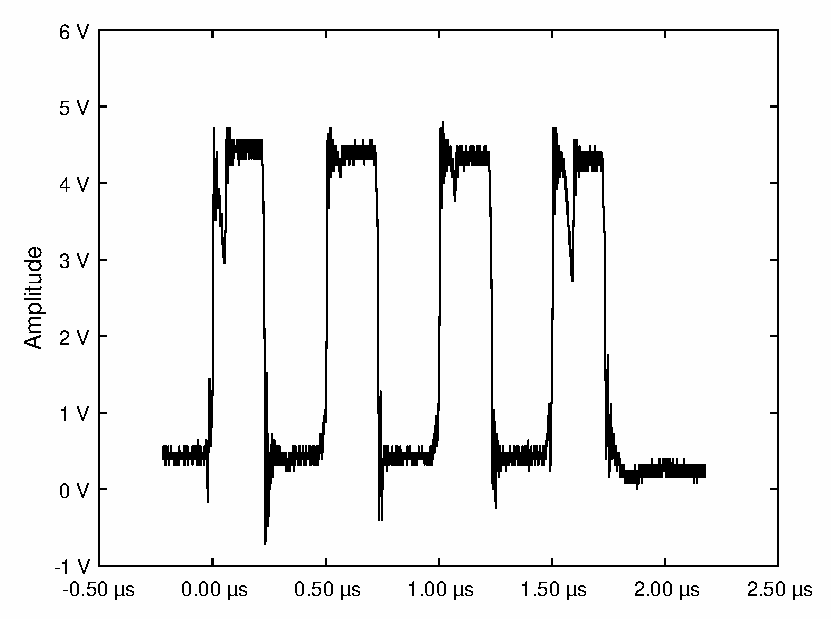
\includegraphics[width=\textwidth, trim= 0mm 0mm 0mm 0mm, clip=true]{images/tests/tx/2MHz-TX.eps}%docu
    	\caption{negatives xDSL Signal mit 2 MHz Ansteuerung}
	    \label{fig:tx2s}
	\end{subfigure}%
    \hfil %add desired spacing between images, e. g. ~, \quad, \qquad, \hfill etc.
    %(or a blank line to force the subfigure onto a new line)
    \begin{subfigure}[t]{0.31\textwidth}
    	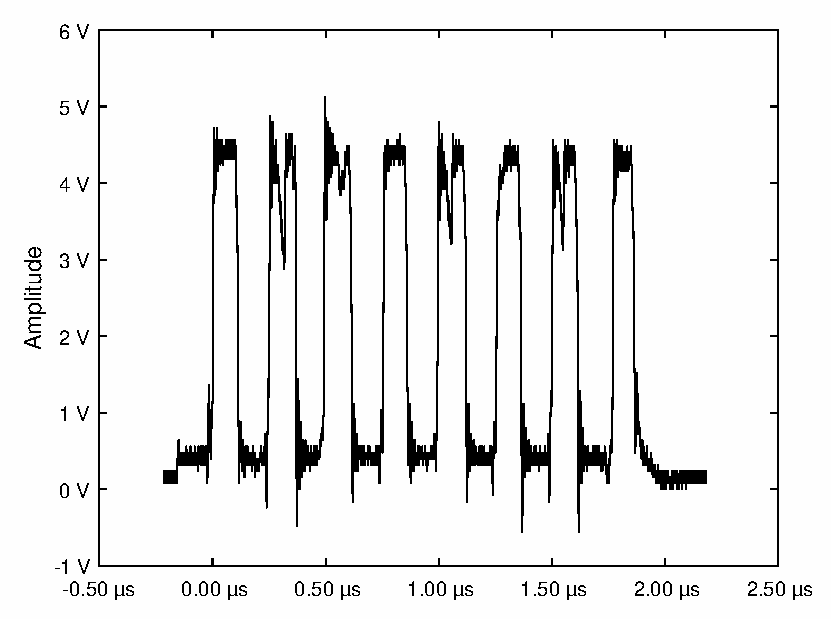
\includegraphics[width=\textwidth, trim= 0mm 0mm 0mm 0mm, clip=true]{images/tests/tx/4MHz-TX.eps}%docu
    	\caption{negatives xDSL Signal mit 4 MHz Ansteuerung}
	    \label{fig:tx4s}
    \end{subfigure}
    \hfil %add desired spacing between images, e. g. ~, \quad, \qquad, \hfill etc.
    %(or a blank line to force the subfigure onto a new line)
    \begin{subfigure}[t]{0.31\textwidth}
    	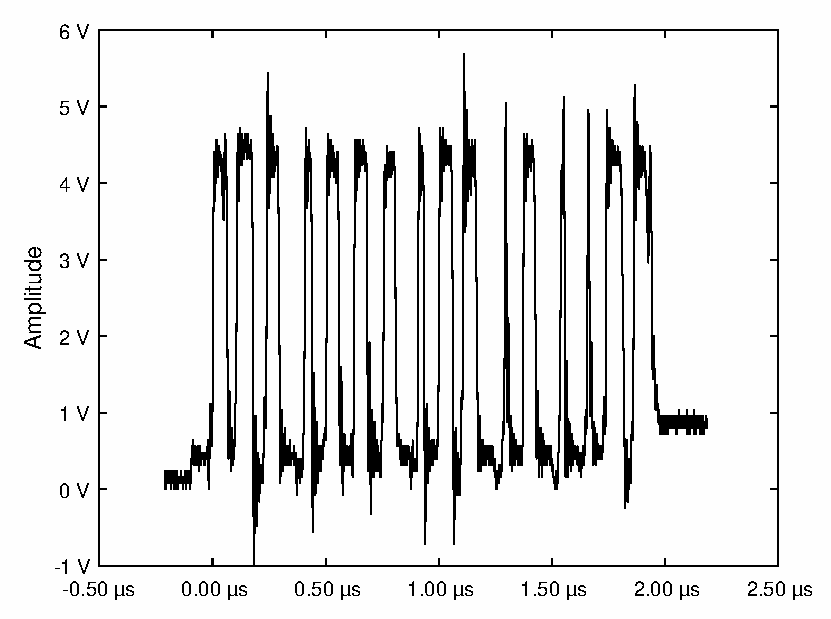
\includegraphics[width=\textwidth, trim= 0mm 0mm 0mm 0mm, clip=true]{images/tests/tx/8MHz-TX.eps}%docu
    	\caption{negatives xDSL Signal mit 8 MHz Ansteuerung}
	    \label{fig:tx8s}
    \end{subfigure}
    \hfil
    \begin{subfigure}[t]{0.31\textwidth}
    \centering
    	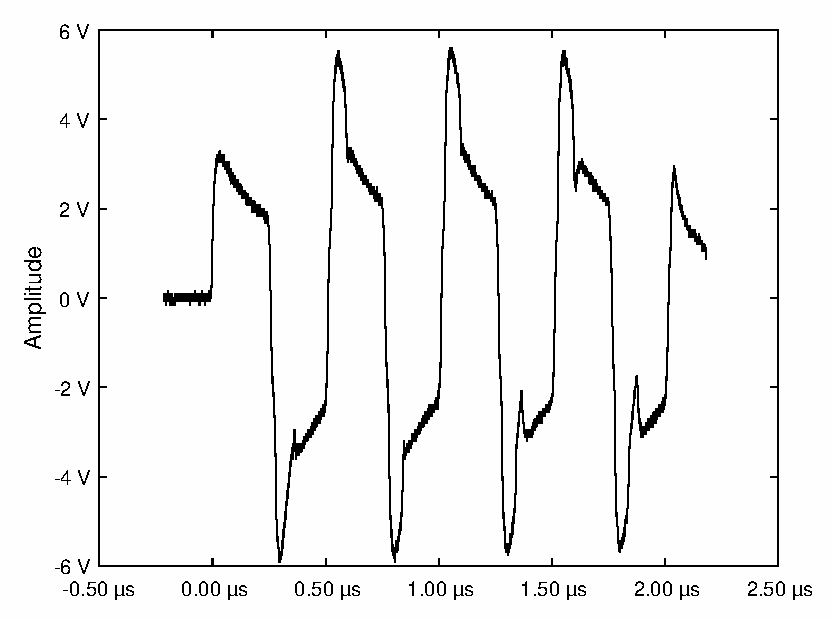
\includegraphics[width=\textwidth, trim= 0mm 0mm 0mm 0mm, clip=true]{images/tests/tx/2MHz-in.eps}%docu
    	\caption{2 MHz Burst}
	    \label{fig:tx2in}
	\end{subfigure}%
    \hfil %add desired spacing between images, e. g. ~, \quad, \qquad, \hfill etc.
    %(or a blank line to force the subfigure onto a new line)
    \begin{subfigure}[t]{0.31\textwidth}
    	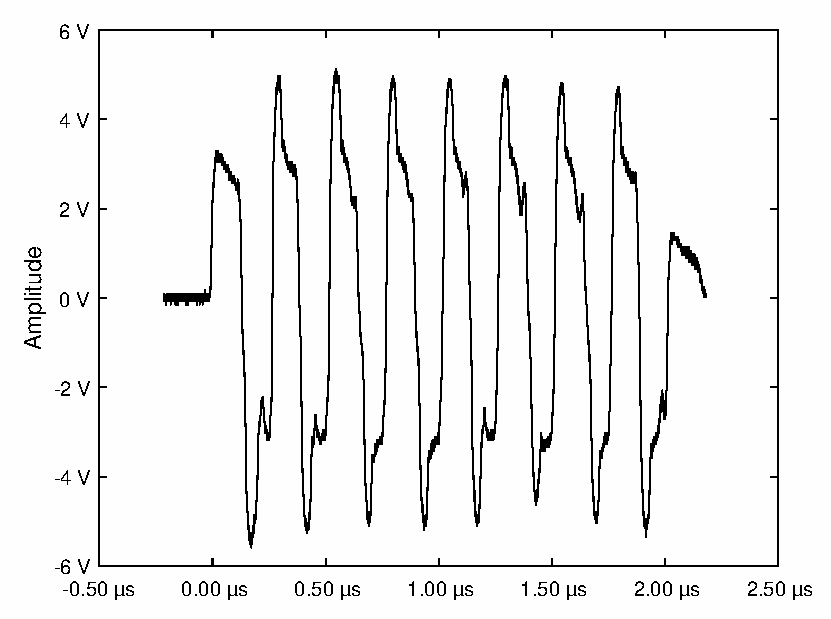
\includegraphics[width=\textwidth, trim= 0mm 0mm 0mm 0mm, clip=true]{images/tests/tx/4MHz-in.eps}%docu
    	\caption{4 MHz Burst}
	    \label{fig:tx4in}
    \end{subfigure}
    \hfil %add desired spacing between images, e. g. ~, \quad, \qquad, \hfill etc.
    %(or a blank line to force the subfigure onto a new line)
    \begin{subfigure}[t]{0.31\textwidth}
    	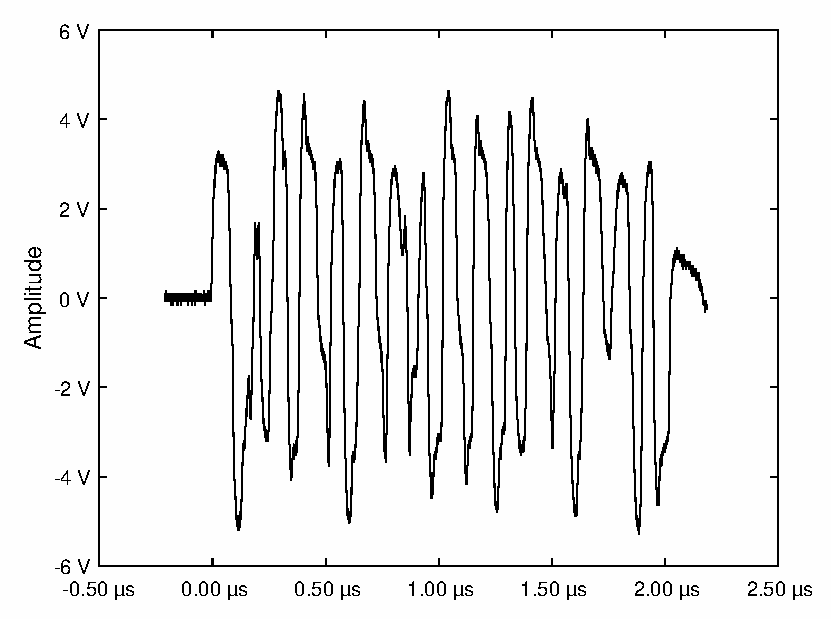
\includegraphics[width=\textwidth, trim= 0mm 0mm 0mm 0mm, clip=true]{images/tests/tx/8MHz-in.eps}%docu
    	\caption{8 MHz Burst}
	    \label{fig:tx8in}
    \end{subfigure}
	\caption{Transmitter Signale vor und nach Wandler}
	\label{fig:tx_measure}
\end{figure}\\
Da Überschwinger in den Ausgangssignalen erkennbar sind, wurde eine nachträgliche Reduzierung des Ringing-Effekts durch 100 $\Omega$ Serienwiderstände an den Eingangssignalen durchgeführt. Dies beeinflusste das Ausgangssignal des xDSL Treibers jedoch nicht. Einbrüche sind an den Ausgangssignalen in \autoref{fig:tx2s}, \autoref{fig:tx4s} und \autoref{fig:tx8s} zu erkennen, was auf eine zu große Last schließen lässt. Die Amplituden der Burst Signale nach dem Transformator brechen je nach Last ein. Zudem sehen diese nicht wie Rechtecksignale oder wie durch die Trägheit der Transformatoren gedacht wie Sinussignale aus, wie in \autoref{fig:tx2in}, \autoref{fig:tx4in} und \autoref{fig:tx8in} ersichtlich wird. Dies deutet auf eine Sättigung der Transformatoren hin, wodurch die maximale Amplitude nicht erreicht werden kann. Die Signalform wird durch die Dominanz der Induktivitäten des Bandpasses verändert, was bei der Simulation nicht berücksichtigt wurde.\\
Ohne weitere Modifikationen ist der Transmitter für die Applikation ungeeignet und sollte daher separat betrachtet werden.
\subsection{Receiver}
Der Receiver wurde als letzte Peripheriekomponente in Betrieb genommen. Dieser ist zentrales Element der Instrumentierung und muss während der Entwicklung angepasst werden, um eine bestmögliche Digitalisierung zu gewährleisten. Auch wenn die Baugruppen separat entwickelt wurden, wird nachfolgend die analoge Signalverarbeitung und die Digitalisierung zusammen betrachtet um die Testzeit zu reduzieren. Zudem zählt das Ergebnis des \ac{snr}s, welches die Genauigkeit des Receivers beschreibt.
\subsubsection*{Testaufbau und -durchführung}
Zunächst wird ein Zähler anstelle der \ac{adc}s in die Logik des \ac{cpld}s implementiert, um softwarebedingte Visualisierungsprobleme zu erkennen und zu beheben. Anschließend wird der PM5139, welcher in \autoref{sec:funktionsgen} beschrieben wird, für die Erzeugung eines Sinussignal genutzt, welches anstelle der Zählwerte visualisiert werden soll. Nachfolgend werden an diesem das Signal in Form, Amplitude und Frequenz geändert, um einen groben Überblick über das Verhalten des Receivers zu erhalten.\\
Nachdem wird zunächst der \ac{snr} bestimmt und optimiert, indem bei einer Trägerfrequenz die Amplitude soweit erhöht wird, bis der maximale Wertebereich des \ac{adc}s ($2^{14}=\pm 8191$) erreicht ist. Dabei wird das Signal über 4096 Messwerte bei 64 \ac{msps} digitalisiert und auf den \ac{pc} gespeichert, woraufhin der \ac{snr} bestimmt wird. Anschließend wird dies für diverse Verstärkungen wiederholt, um Aussagen über das Rauschen des Vorverstärkers zu treffen. Dabei wird der Widerstand $R_G$ des Vorverstärkers nach Bedarf getauscht.\\
Nachdem der \ac{snr} im Verhältnis zur Verstärkung gewählt wurde, wird die Verstärkung über den Frequenzbereich 0,5 bis 10 \ac{mhz} in 500 \ac{khz} Schritten bestimmt. Dabei wird die Amplitude des Signals soweit erhöht, bis der \ac{adc} ausgesteuert wird.
\subsubsection*{Ergebnisse}
Die Zählwerte konnten nach Anpassung der Datentypen der QT-Software visualisiert werden. Für das Sinussignal hingegen musste die Verilog Syntax genauer betrachtet werden. Dabei ergab sich, dass die geplante Biterweiterung von 14 auf 16 Bit fehlerhaft war. Dies konnte durch den Befehl $\$signed()$ kompensiert und das RF-Signal erfolgreich visualisiert werden.\\
Da der \ac{snr} nur 59,55 \ac{db} betrug, wurde der Verstärkungsfaktor über den Widerstand $R_G$ angepasst. Die Ergebnisse werden in \autoref{tab:snr_results} auf Seite \pageref{tab:snr_results} zusammengefasst. Zudem wurden die Eingänge des \ac{adc}s kurzgeschlossen und das \ac{snr} durch die maximal mögliche Auflösung ermittelt. Dabei stellte sich ein Wert von 74,45 \ac{db} heraus, welcher als mögliches Limit des \ac{adc}s zu Verfügung steht. Es wurde sich für eine Verstärkung von 13,3 dB bei einer Trägerfrequenz von 2 \ac{mhz} entschieden, da diese einen \ac{snr} 69,87 dB bieten kann. Der Widerstand $R_G$ wurde folglich auf 100 $\Omega$ erhöht, die Samplingfrequenz angepasst und der \ac{snr} bestimmt. Dabei ergab sich eine Abweichung von 0,1 \ac{db}, welche durch Messungenauigkeiten entstehen kann.
\begin{figure}[h!]
\centering
	\begin{subfigure}[t]{0.48\textwidth}
    \centering
    	\includegraphics[width=\textwidth, trim= 0mm 0mm 0mm 0mm, clip=true]{images/tests/bandpassUin}%docu
    	\caption{benötigte Eingangsspannung des Receivers für die maximale Aussteuerung des \ac{adc}-Eingangs}
	    \label{fig:pcb_top}
	\end{subfigure}%
    \hfil %add desired spacing between images, e. g. ~, \quad, \qquad, \hfill etc.
    %(or a blank line to force the subfigure onto a new line)
    \begin{subfigure}[t]{0.48\textwidth}
    	\includegraphics[width=\textwidth, trim= 0mm 0mm 0mm 0mm, clip=true]{images/tests/bandpassDB}%docu
    	\caption{Verstärkung der gesamten Receivermoduls}
	    \label{fig:pcb_bottom}
    \end{subfigure}
	\caption{Filtercharakteristik des Receivermoduls}
	\label{fig:bp_filter}
\end{figure}\\
Der Bandpass wurde nach Bestimmung des \ac{snr} erfasst, indem die Eingangsfrequenz von 0,5 \ac{mhz} bis 10 \ac{mhz} in 0,5 \ac{mhz} Schritten verändert wurde. Daraus ergaben sich die Graphen in \autoref{fig:bp_filter}. Es ist zu erkennen, dass das Filterverhalten von dem gewollten Verhalten abweicht. Jedoch verstärkt der Receiver Signale um 2 \ac{mhz} um rund 13 \ac{db}, Singale um 4 \ac{mhz} um rund 11 \ac{db} und Singale um 8 \ac{mhz} um rund 11 \ac{db}, was einen Verstärkungsfaktor von 4,4 und 3,5 entspricht.
\begin{table}[h!]
\centering
\caption{\acs{snr} in Abhängigkeit der Verstärkung und Widerstand $R_G$}
\label{tab:snr_results}
\begin{tabular}{r|>{\centering}p{2.6cm}|>{\centering}p{2.3cm}|>{\centering}p{2.3cm}|>{\centering}p{2.3cm}|c}
\textbf{$R_G$} & \textbf{Verstärkungs-faktor} & \textbf{Verstärkung} & \textbf{Eingangs-amplitude} & \textbf{Sampling-frequenz} & \textbf{\ac{snr}} \\
\cline{1-6}
8,6 $\Omega$	& 20,00 & 26,0 \ac{db} & 100 mV\ac{pp} & 64 \ac{msps} & 59,96 \ac{db} \\ 
39 $\Omega$ 	& 9,09	& 19,2 \ac{db} & 220 mV\ac{pp} & 64 \ac{msps} & 66,61 \ac{db} \\
82 $\Omega$ 	& 5,60	& 14,9 \ac{db} & 357 mV\ac{pp} & 64 \ac{msps} & 68,96 \ac{db} \\
100 $\Omega$ 	& 4,62	& 13,3 \ac{db} & 433 mV\ac{pp} & 64 \ac{msps} & 69,87 \ac{db} \\
150 $\Omega$ 	& 3,45	& 10,7 \ac{db} & 580 mV\ac{pp} & 64 \ac{msps} & 71,30 \ac{db} \\
220 $\Omega$ 	& 2,06	& 6,3  \ac{db} & 970 mV\ac{pp} & 64 \ac{msps} & 71,86 \ac{db}
\end{tabular}
\end{table}
\subsection{Signalintegrität und Kopplungen}
Um die induktive Entkopplung der analogen Komponenten und somit die Stabilität der Spannungsversorgung im Betrieb sicherzustellen muss dieser Test durchgeführt werden. Gleichzeit kann mit diesem das Nachschwingverhalten von digitalen Signalen überprüft werden. Das Ringing stellte eine zusätzlich Belastung der Spannungsversorgung dar und führt zur Entstehung von Störsignalen, welche abgestrahlt werden können. Daher werden diese detektiert um eine Optimierung der Instrumentierung zu ermöglichen.
\subsubsection*{Testaufbau und -durchführung}
Zunächst wird mit dem Oszilloskop HMO3524 die Welligkeit aller Spannungsversorgungen im Betrieb gemessen und untersucht. Dabei kann das Spektrum untersucht werden um Rückschlüsse auf die Störquellen zu erhalten. Wenn Frequenzen um 64 \ac{mhz} oder einem vielfachen davon im Spektrum sichtbar sind, wird eine Nahfeldsonde benötigt, um Rückschlüsse über den Entstehungsort zu erhalten. Zudem kann eine Strommesszange in Verbindung mit einen Spektrum-Analysator verwendet werden, um Frequenzen auf der Zuleitung und dem Anschluss zur Sonde zu erkennen. Dabei wird ein \ac{usb} Kabel durch die Strommesszange geführt und das Spektrum visualisiert.
\subsubsection*{Ergebnisse}
Die \ac{fft} Funktion des Oszilloskop HMO3524 zeigte einen deutlichen Anstieg des 64 \ac{mhz} Signals und der zweiten Oberwelle bei 192 \ac{mhz}. Daher wurde eine Nafeldsonde an den Testpunkten wie in der \autoref{fig:measurepoints} positioniert und das Spektrum von einen bis 640 \ac{mhz} mit dem Spectrum Analyzer FSL3 aus \autoref{sec:analyzer} aufgenommen. Die Ergebnisse sind in \autoref{fig:signal_int} aufgeführt.
\begin{figure}[h!]
	\centering
	\begin{subfigure}[t]{0.42\textwidth}
    \centering
\begin{annotatedFigure}
	{\includegraphics[page=4,width=1\textwidth, trim= 0mm 0mm 0mm 0mm, clip=true]{images/pcb/Job2.PDF}}
	\draw[line width=1.0mm] (0.2838,0.048) -- (0.3324,0.048) node[fill=black,thick,shape=circle,inner sep=2pt,font=\sffamily,text=white] {a};
	\draw[line width=1.0mm] (0.1627,0.082) -- (0.2101,0.044) node[fill=black,thick,shape=circle,inner sep=2pt,font=\sffamily,text=white] {b};
	\draw[line width=1.0mm] (0.3721,0.162) -- (0.4214,0.1974) node[fill=black,thick,shape=circle,inner sep=2pt,font=\sffamily,text=white] {c};
	\draw[line width=1.0mm] (0.1655,0.458) -- (0.1655,0.406) node[fill=black,thick,shape=circle,inner sep=2pt,font=\sffamily,text=white] {d};
	\draw[line width=1.0mm] (0.0543,0.486) -- (0.0543,0.432) node[fill=black,thick,shape=circle,inner sep=2pt,font=\sffamily,text=white] {e};
	\draw[line width=1.0mm] (-0.0037,0.404) -- (0.0543,0.404) node[fill=black,thick,shape=circle,inner sep=2pt,font=\sffamily,text=white] {f};
	\draw[line width=1.0mm] (0.4125,0.534) -- (0.4742,0.534) node[fill=black,thick,shape=circle,inner sep=2pt,font=\sffamily,text=white] {g};
	\draw[line width=1.0mm] (0.2345,0.466) -- (0.2962,0.466) node[fill=black,thick,shape=circle,inner sep=2pt,font=\sffamily,text=white] {h};
	\draw[line width=1.0mm] (0.122,0.217) -- (0.122,0.174) node[fill=black,thick,shape=circle,inner sep=2pt,font=\sffamily,text=white] {i};
	\draw[line width=1.0mm] (0.122,0.221) -- (0.122,0.274) node[fill=black,thick,shape=circle,inner sep=2pt,font=\sffamily,text=white] {j};
	\draw[line width=1.0mm] (0.1889,0.124) -- (0.1306,0.124) node[fill=black,thick,shape=circle,inner sep=2pt,font=\sffamily,text=white] {k};
	\draw[line width=1.0mm] (0.2099,0.124) -- (0.2099,0.092) node[fill=black,thick,shape=circle,inner sep=2pt,font=\sffamily,text=white] {l};
	\draw[line width=1.0mm] (0.1789,0.144) -- (0.2406,0.144) node[fill=black,thick,shape=circle,inner sep=2pt,font=\sffamily,text=white] {m};
	\draw[line width=1.0mm] (0.2862,0.144) -- (0.3434,0.144) node[fill=black,thick,shape=circle,inner sep=2pt,font=\sffamily,text=white] {n};
	\draw[line width=1.0mm] (0.1705,0.2456) -- (0.2122,0.2236) node[fill=black,thick,shape=circle,inner sep=2pt,font=\sffamily,text=white] {o};
\end{annotatedFigure}
    \caption{Ground Plane und Komponenten auf der Platinenoberseite - Richtung der Nahfeldsonde}
    \label{fig:system_layout}
    \end{subfigure}%
    \hfil
    \begin{subfigure}[t]{0.42\textwidth}
    \centering
    \begin{annotatedFigure}
	{\includegraphics[page=5,width=1\textwidth, trim= 0mm 0mm 0mm 0mm, clip=true]{images/pcb/Job2.PDF}}
	\draw[line width=1.0mm] (0.1505,0.2456) -- (0.1922,0.2236) node[fill=black,thick,shape=circle,inner sep=2pt,font=\sffamily,text=white] {p};
	\draw[line width=1.0mm] (0.5074,0.206) -- (0.4768,0.178) node[fill=black,thick,shape=circle,inner sep=2pt,font=\sffamily,text=white] {q};
	\draw[line width=1.0mm] (0.226,0.1296) -- (0.276,0.1296) node[fill=black,thick,shape=circle,inner sep=2pt,font=\sffamily,text=white] {r};

	\draw[line width=1.0mm] (0.2037,0.534) -- (0.256,0.534) node[fill=black,thick,shape=circle,inner sep=2pt,font=\sffamily,text=white] {s};
\end{annotatedFigure}
	\caption{Power Plane und Komponenten auf Platinenunterseite - Richtung der Nahfeldsonde}
    \end{subfigure}
    \caption{Messpunkte der Nahfeldsonde für die Signalintegrität in \autoref{sec:signal_db}}
    \label{fig:measurepoints}
\end{figure}\\
Nach Betrachtung der Ergebnisse ergab sich, dass die Oberwellen eine höhere Amplitude als das 64 \ac{mhz} Signal aufweisen. Daher wird vermutet, dass das Filter zwar wirkt, jedoch durch eine schlechte Impedanz an Wirkung verliert. Die Vermutung wurde durch eine Spektralanalyse mit einer Strommesszange an dem nicht geschirmten \ac{usb} Kabel bestätigt, da 64 \ac{mhz} und dessen Oberwellen auf der Versorgungsleitung erkennbar sind (\autoref{fig:strom_spannung}). Weiterhin wurde die Signalleitung zur Sonde (\autoref{fig:strom_sonde}) mit der Strommesszange gemessen und das Spektrum wies die gleichen Amplituden auf. Dies lässt den eindeutig Schluss zu, dass ein Ground-bouncing vorherrscht. Somit wurde die Anordnung der Bypass-Kondensatoren des \ac{adc}s näher betrachtet. Der Abstand zwischen dem digitalen Versorgungspin und dem Bypass beträgt rund 2 mm, wischen den analogen Versorgungspins und den Bypass Kondensatoren 3 und 4,4 mm. Die Faustformel besagt, dass 1 mm Leiterbahnweg einen 1 nH entspricht. Somit ergibt sich die \autoref{tab:imp_caps}. Die Traget-Impedanz sollte bei 0,01 $\Omega$ liegen, damit die Filtercharakteristik auch bei den Oberwellen bis 6,4 \ac{ghz} wirken kann.
\newcolumntype{L}[1]{>{\RaggedRight\hspace{0pt}}p{#1}}
\newcolumntype{R}[1]{>{\RaggedLeft\hspace{0pt}}p{#1}}
\begin{table}[h!]
\centering
\caption{Impedanz in Abhängigkeit von der Frequenz und dem Abstand}
\label{tab:imp_caps}
\begin{tabular}{r|R{2,4cm}|R{2,4cm}|R{2,4cm}|R{2,4cm}}
\textbf{Frequenz} & \textbf{Impedanz bei 0,2 mm} & \textbf{Impedanz bei 2 mm} & \textbf{Impedanz bei 3 mm} & \textbf{Impedanz bei 4,4 mm}\\
\cline{1-5}
64 \ac{mhz} & 0,08 $\Omega$ & 0,8 $\Omega$ & 1,2  $\Omega$ & 1,77  $\Omega$ \\
128 \ac{mhz} & 0,16 $\Omega$ & 1,6 $\Omega$ & 2,41  $\Omega$ & 3,54  $\Omega$ \\
192 \ac{mhz} & 0,24 $\Omega$ & 2,41 $\Omega$ & 3,62  $\Omega$ & 5,31  $\Omega$ \\
256 \ac{mhz} & 0,32 $\Omega$ & 3,21 $\Omega$ & 4,83  $\Omega$ & 7,07  $\Omega$ \\
320 \ac{mhz} & 0,40 $\Omega$ & 4,02 $\Omega$ & 6,03  $\Omega$ & 8,85  $\Omega$ \\
512 \ac{mhz} & 0,64 $\Omega$ & 6,43 $\Omega$ & 9,65 $\Omega$ & 14,15  $\Omega$ \\
1024 \ac{mhz} & 1,28 $\Omega$ & 12,86 $\Omega$ & 19,30 $\Omega$ & 28,31  $\Omega$
\end{tabular}
\end{table}\\
Aus \autoref{tab:imp_caps} ist ersichtlich, dass die Traget-Impedanz von 0,01 $\Omega$ nicht erreicht wurde. Daher ist eine Kompensation des Ground-bouncing Effekts ohne ein Redesign nicht realisierbar.
\subsection{Demodulierung}\label{sec:demodulation_results}
Aus Zeitgründen konnte die Logik der Demodulierung nicht mit der aktuellen Hardware getestet werden. Jedoch wurde diese in der Bachelor Thesis von Herrn A. Rehn 2014 deklariert und ausführlich getestet, wodurch diese nachträglich implementiert werden muss.
\clearpage
\section{Integrationstest}\label{sec:inttest}%(Integration-Test)
\begin{figure}[h!]
\centering
	\begin{subfigure}[b]{0.499\textwidth}
    \centering
    	\includegraphics[page=3,width=\textwidth, trim= 65mm 5mm 65mm 0mm, clip=true]{images/pcb/Job2.PDF}%docu
    	\caption{Oberseite der Dopplerinstrumentierung}
	    \label{fig:pcb_top}
	\end{subfigure}%
    \hfil %add desired spacing between images, e. g. ~, \quad, \qquad, \hfill etc.
    %(or a blank line to force the subfigure onto a new line)
    \begin{subfigure}[b]{0.499\textwidth}
    	\includegraphics[page=2, width=\textwidth, trim= 65mm 5mm 65mm 0mm, clip=true]{images/pcb/Job2.PDF}%docu
    	\caption{Unterseite der Dopplerinstrumentierung}
	    \label{fig:pcb_bottom}
    \end{subfigure}
    \hfil
    ~
    \begin{subfigure}[b]{1\textwidth}
    	\includegraphics[width=\textwidth, trim= 230mm 155mm 0mm 65mm, clip=true]{images/pcb/WP_20150709_002}
    	\caption{\ac{pcb} der Dopplerinstrumentierung (vorne bestückt, hinten nicht bestückt)}
		\label{fig:3Dpcb}
    \end{subfigure}
	\caption{Ergebniss des \acs{pcb}-Layouts}\label{fig:pcb}
\end{figure}
Nachdem die grundlegenden Funktionalitäten verifiziert wurden, konnte das System in Betrieb genommen werden. Wie in \autoref{sec:demodulation_results} beschrieben erfolgt keine Demodulierung des RF-Signals. Hingegen werden 14-Bit RF-Signale durch die geschriebene QT-Software erfolgreich dargestellt. Die OnTheFly Änderung von Parametern über die QT-Software funktioniert nur bei der Starttiefe der \ac{roi}. Dies deutet auf ein Problem der Logik des \ac{cpld}s hin, da der \ac{spi} Datentransfer wie erwartet arbeitet und aktuell alle Parameter transferiert werden.\\
Durch die mangelnde Funktionalität des Transmitters, konnte kein Transducer erfolgreich in Betrieb genommen werden. Jedoch können die Signale des Transmitters durch den Receiver digitalisiert und mit der QT-Software dargestellt werden.\\
Durch die verspätete Lieferung des Gehäuses konnten keine Aussparungen für das Frontblech des Gehäuses durchgeführt werden. Dies beeinträchtigt die Funktionalität der Applikation jedoch nicht, wodurch dies nachträglich durchgeführt werden kann. Zudem sind die vorgesehen Montagelöcher für gängige Schrauben und Abstandshalter zu klein, wodurch eine Montage erschwert wird.\\
Das realisierte System läuft grundsätzlich über einen Testzeitraum von 10 Minuten stabil. Dabei treten Darstellungsfehler auf, welche auf ein fehlendes Byte während eines Frames hindeuten. Dies wird ersichtlich, wenn das \ac{fifo} des \ac{cpld}s nicht genügend Samples zu Verfügung stellen kann. Durch das fehlende Byte wird der 16-Bit Wert geshiftet, was einen Offset und ein Skalierungsproblem zur Folge hat.\\
Eine Synchronisierung wischen \ac{pc} und LPC4337 wurde nicht realisiert, da der Fokus auf der Umsetzung der grundlegenden Funktion lag. Daher benötigt der Test-\ac{pc} 18,8 MB Arbeitspeicher und rund 23 bis 48 \% der Intel I5 Rechenleistung.
\chapter{Diskussion und Ausblick}
In diesem Kapitel wird das Erreichte zunächst in \autoref{sec:discussion_results} zusammengefasst. Aufkommende Fragen während der Testdurchführung und der Testergebnisse werden anschließend in \autoref{sec:discussion_testresults} analysiert und ein Fazit durch Schlussfolgerungen dargestellt. Weiterhin wird die Realisierung der Anforderungen in \autoref{sec:discuss_all} und deren Umsetzung in \autoref{sec:discuss_tasks} analysiert und objektiv bewertet. Abgeschlossen wird das Kapitel, indem in \autoref{sec:futurework} Verbesserungspotentiale aufgezeigt und mögliche Weiterentwicklungen des Systems und dessen Module erbracht werden.
\section{Zusammenfassung der Ergebnisse}\label{sec:discussion_results}
Im Rahmen der vorliegenden Arbeit wurde eine Dopplerinstrumentierung entwickelt, welche das Messen von Ultraschall Dopplerschiebefrequenzen bedingt erlaubt. Die aus dem Messverfahren resultierenden M-Mode und Doppler Spektrogramm Darstellungen zu realisieren gelang in den zur Verfügung stehenden Zeitraum nicht. Dafür konnten die grundlegenden Funktionen für die Realisierung des Messverfahrens, sowie der Visualisierung umgesetzt werden. Eine Echtzeitvisualisierung der RF-Daten konnte erfolgreich auf dem \ac{pc} dargestellt werden, was die Grundlage für die Visualisierung der Graphen bildet und die Möglichkeiten des Systems zeigt. Durch die Nutzung eines Embedded Systems kann die analoge durch eine digitale Demodulierung ersetzt werden, was nicht nur kosteneffizienter ist, sondern mehr Informationen pro Hardware Channel und Digitalisierung bietet. Die entwickelte Instrumentierung    kann somit als Alternative für die Erkennung von Embolien dienen, wenn die erkannten Probleme behoben und die Software komplettiert ist.
\section{Diskussion der Testergebnisse und der Testdurchführung}\label{sec:discussion_testresults}
\subsubsection*{Transmitter}
Der Transmitter erfüllt die Anforderungen nicht, da er die zu nutzenden Frequenzen nicht konstant und 8 \ac{mhz} gar nicht treiben kann. Die Hardware weicht soweit von der Simulation ab, dass es in der zu Verfügung stehenden Zeit unmöglich war, einen plausiblen Grund für das Versagen des xDSL Treibers zu finden. Aus wirtschaftlichen und zeitlich Gründen sollten daher Alternativen bevorzugt werden. Weiterhin muss der Transmitter während der Brustphase von dem Receiver entkoppelt werden, da die Induktivitäten des Bandpassfilters die zu sendende Signalform beeinflussen. Dies könnte \ac{zb} durch einen SPDT Schalter erfolgen.
\section{Diskussion zur Einhaltung aller Anforderungen}\label{sec:discuss_all}
\subsubsection*{Software- und Hardwareanforderungen}
Die Anforderungen an die Energieversorgung sind nach einer Anpassung der ersten Spannungsreduzierung erfolgreich umgesetzt wurden. Der integrierte Verpolschutz schützt das System erfolgreich bei verpolten Eingängen und sollte beibehalten werden. Die genierten Spannungen unterliegen keinen Einbrüchen. Der Abstand der Bypasskondensatoren zu den \ac{ic}s ist zu groß für die bei dieser Applikation vorkommenden Frequenzen und deren Oberwellen. Somit ist das Filterverhalten und die induktive Entkopplung nur bei geringeren Frequenzen gewährleistet. Dies macht sich durch Brummspannung von $\pm$ 5 bis 10 mV der Spannung bemerkbar, wodurch das \ac{snr} reduziert wird. Es ist davon auszugehen, dass ein Ground-bouncing mit der Taktfrequenz des \ac{adc} \ac{ic}s verursacht wird, da das Filterverhalten mangelhaft ist. Eine Kompensation des Problems kann dabei den möglichen \ac{snr} erhöhen wodurch Amplituden im $\mu$V Bereich unterschieden werden können. Die Software- und Hardwareanforderungen wurden teilweise realisiert. Dabei konnten die \ac{emi} Richtlinien durch das vorkommende Nachschwingverhalten der Spannungsversorgung nicht eingehalten werden und eine Visualisierung des aktuell angeschlossenen Transducers nicht realisiert. 
\subsubsection*{Systemanforderungen}
Das Netzteil GXM60-19A04 ist nach EN60601 zugelassen, wodurch dieses in medizinischen Bereichen genutzt werden kann. Weiterhin besitzt die Platine einen NXP LPC4337, welcher als Kern einen asymmetrischen ARM\SymbReg Cortex\SymbReg-M4/M0 besitzt und ausreichend Reserven für nachträgliche Implementierungen bietet. Die \ac{usb}-micro Buchse wurde vorgesehen, ist jedoch durch einen Layoutfehler nicht nutzbar und wurde durch eine direkte Anbindung eines \ac{usb}-Kabels ersetzt. Bei der Montage der \ac{usb}-micro Buchse muss beanstandet werden, dass diese sehr schwer zu positionieren ist. Ein alternatives Package der Buchse könnte die Montage drastisch vereinfachen.
\subsubsection*{Benutzeranforderungen}
Eine Umsetzung der Benutzeranforderungen erfolgte zielstrebig. Das System besteht aus einer Platine, welche über eine QT-Software angesteuert wird. Dabei ist die QT-Plattform unter Linux Distributionen und Microsoft\SymbC Windows\SymbReg lauffähig. Jedoch können durch die verringerte Funktionsfähigkeit des Transmitters keine Transducer im Frequenzbereich von 2, 4 und 8 \ac{mhz} betrieben werden. Außerdem konnte durch Zeitmangel keine Demodulierung implementiert werden, wodurch keine I/Q-, sondern RF-Werte übertragen werden. Die implementierten Schnittstellen erlauben 96 I/Q-Werte pro \ac{prf} zu übertragen, wodurch die Anforderung der Datenübertragung teilweise realisiert werden konnte.

\section{Diskussion der Ergebnisse bzgl. der Aufgabenstellung}\label{sec:discuss_tasks}
Durch die Nutzung neuer \ac{ic}s, welche für weitere Entwicklungen Reserven bieten müssen, verlagerte sich der Schwerpunkt der Arbeit von der Applikation hin zur Hardware und deren Inbetriebnahme. Aus diesem Grund bietet diese Arbeit keinen implementierten Algorithmus zur eindeutigen Emboliedetektion und spricht diese Thematik nicht an. Mit der Inbetriebnahme der neuen \acs{ic}s und deren Logik, welche die realisierte Software und Schnittstellen beinhaltet, wurde der Grundstein für eine möglichst detailliere Emboliedetektion gelegt, indem die Möglichkeiten des Systems in dieser Arbeit dargestellt sind. Eine Ansteuerung der Transducer konnte durch die mangelhafte Transmitterschaltung nicht realisiert werden, wodurch keine Erfassung von Ultraschallsignalen möglich ist. Die Datenrate für die Übertragung der I/Q-Signale konnte drastisch erhöht und eine \ac{gui}-Implementierung ohne M-Mode und Spektrogramm Algorithmen erarbeitet werden.\\
Das entwickelte System kann als Grundlage für die Weiterentwicklung der Applikation verwendet werden, wenn die Erkenntnisse der Arbeit umgesetzt werden.
\section{Verbesserungspotentiale und Ausblick}\label{sec:futurework}
\subsubsection{Spannungsversorgung}

\subsubsection{Receiver}
\subsubsection{Steuerung und Demodulierung}
\subsubsection{Kommunikation und Datenübertragung}
\subsubsection{Visualisierung}
%
%
%

\subsubsection{Layout und Hardware}
\subsubsection{Logik und Software}

\subsubsection{Kostenreduzierung}
Da im Rahmen dieser Arbeit eine Basis für eine Dopplerinstrumentierung entwickelt wurde, und die nötigten Implementierungen der Hard- und Software schwer Abzuschätzen waren, wurde sich für das größte \ac{cpld} und einen der größten asymmetrischen ARM\SymbReg Cortex\SymbReg-M4/M0 \ac{mcu}s entschieden. Diese können nach Bedarf durch kleinere Chips ersetzt werden. So stehen \ac{zb} für den NXP LPC4337 pinkompatible Alternativen mit ARM\SymbReg Cortex\SymbReg-M3 Kern (LPC1800 Serie) oder kleinere (LPC4300 Serie) zu Verfügung. Die \ac{lut} Anzahl des \ac{cpld}s hingen ist pinabhängig, wodurch ein Redesign nötig ist. 

\chapter*{Schlusswort}
\addcontentsline{toc}{chapter}{Schlusswort}
Ich möchte mich bei allen bedanken, die zu dieser Arbeit beigetragen haben. Besonders möchte ich mich bei meinen betreuenden Professor Herr \gutachterA \ für die Betreuung und die Überlassung des Themas bedanken. Zudem Herrn \gutachterB, welcher mir selbstlos in den Themengebieten \ac{emi} und Signalintegrität zur Seite stand. Des weiteren Herrn Dr.-Ing. Gert Schönfelder für Inspirationen zur Realisierung der Hardware, sowie {\href{mailto:schilling@hs-ulm.de}{Herrn Schilling-Kästle} für die schnelle Umsetzung des \ac{pcb} Layouts, der Bestellung der \ac{bom} und seiner beispiellosen Unterstützung. Hiermit möchte ich mich auch bei meinen Eltern, meiner Schwester und meiner Freundin Nadine für Ihre Unterstützung sowie das Korrekturlesen der Arbeit bedanken.